\section{Beyond the SM: Leptoquark physics}

As claimed in chapter \ref{ch:chapter1}, the main motivation for introducing leptoquarks is that they provide an explanation for LFU violation, as hinted by experimental $B$-meson decay anomalies \cite{lhcb_measurement,lhcbcollaboration2021test}. Although there is a plethora of combined explanations for these anomalies in the literature (see for instance \cite{buttazzo_b-physics_2017, calibbi_effective_2015, bhattacharya_simultaneous_2015, alonso_lepton_2015}), mainly within the Effective Field Theory (EFT) framework, many of them exhibit serious issues such as a breakdown of the perturbative expansion, missing ultra-violet (UV) completion, and excess tuning of parameters \cite{di_luzio_maximal_2018}. Moreover, few models are consistent with high transverse momentum ($p_T$) constraints, as outlined in \cite{faroughy_confronting_2017, greljo_high-p_tdilepton_2017}, and other experimental (non-)observations \cite{di_luzio_gauge_2017}. Nonetheless, the literature has singled out a vector leptoquark in the $(3,1,2/3)$ representation of the SM gauge group coupled mainly to third-generation fermions as a simple addition to the SM which explains all anomalies and is consistent with low-energy data \cite{buttazzo_b-physics_2017}. A crucial feature of this representation is the absence of down-quark-to-neutrino or up-quark-to-charged-lepton transitions \cite{di_luzio_gauge_2017}. In other explanations for the anomalies, suppression of these interactions requires stringent and often unnatural constraints on the model. However, the inclusion of a massive vector field requires a UV completion. This section reviews a subset of the literature devoted to embedding the $(3,1,2/3)$ leptoquark in suitable UV completion.

There are two ways a UV-complete theory may produce massive vectors: composite dynamics \cite{barbieri_anomalies_2016} or a spontaneously broken gauge symmetry. The former approach although plausible and theoretically consistent with precision electroweak measurements, it exhibits renormalisation issues \cite{di_luzio_gauge_2017}. Hence, the latter approach is followed. Consider the gauge group $G = SU(4)\times SU(3)' \times SU(2)_L \times U(1)'$. The model arising from this gauge structure is known as the 4321 model, due to the degree in each factor, and is constructed following a bottom-up approach. The experimental anomalies require the following effective interaction terms with SM fermions:
\begin{equation}\label{eq:LQ-fermion-lag}
    \mathcal{L} \supset \frac{g_U}{\sqrt{2}} U_{1}^{\mu,\alpha} \qty[\beta_{L}^{ij}\overline{q}_L^{i,\alpha}\gamma_\mu \ell^{j}_{L} + \beta_{R}^{ij}\overline{d}_R^{i,\alpha}\gamma_\mu e^{j}_{R}] + \mathrm{h.c.},
\end{equation}
where $U_1^\mu$ is the vector leptoquark, $q_L (\ell_L)$ denotes left-handed quark (lepton) doublets, $d_R (e_R)$ denotes right-handed down-type quark (charged-lepton) singlets, $i,j\in\{1,2,3\}$ are family indexes, $\alpha\in \{1,2,3\}$ are $SU(3)_c$ colour indices and $\beta^{ij}_{L/R}$ are complex matrices. These terms in turn fix the SM representation for the $U_1$ vector as $(3,1,2/3)$. The minimal group $G_{\mathrm{min}} \supset G_{\mathrm{SM}}$ that contains generators transforming under this representation is \cite{baker_high_2019}, 
\begin{equation}\label{eq:G-min1}
    G_{\mathrm{min}} = SU(4) \times SU(2)_L \times U(1)_{T_R^3}.
\end{equation}
$G_{\mathrm{min}}$ is obtained as a subgroup of the Pati-Salam group \cite{pati_lepton_1974}, $$ G_{\mathrm{PS}} = SU(4) \times SU(2)_L \times SU(2)_R,$$ by defining $U(1)$ to be the subgroup of $SU(2)_R$ defined by the diagonal (electric-charge neutral) generator $T_R^3$. However, the minimal group from \eqref{eq:G-min1} constraint the coupling constants so much that there is no freedom to comply with low-energy and high-energy data \cite{baker_high_2019}. This is issue is averted by the next-to-minimal gauge group, $$G = SU(4)\times SU(3)' \times SU(2)_L \times U(1)_{T_R^3}.$$


% On the other hand, there is a purely theoretical perspective presented in \cite{di_luzio_gauge_2017}. The chiral structure of the SM suggests the Pati-Salam (PS) model with gauge structure $$G_{\text{PS}} = SU(4)_{\text{PS}} \times SU(2)_L \times SU(2)_R.$$ However, this model puts the LQ mass close to $100\;\si{TeV}$, meaning it could not explain low-energy LFU violations.

\subsection{Features of the 4321 Model}

It is clear that the 4321 extends the SM group by an extra $SU(4)$ factor. However, the embedding of $G_{\text{SM}}$ in the 4321 group is not that straightforward: the $SU(3)_c$ factor is identified with a diagonal subgroup, namely $$\qty(SU(3)_4 \times SU(3)')_{\mathrm{diag}},$$ where $SU(3)_4\times U(1)_4 \subset SU(4)$. Similarly, $$U(1)_Y = (U(1)_4\times U(1)')_{\mathrm{diag}}.$$ This embedding produces certain relationships between the $G_{\mathrm{SM}}$ generators and those of the larger group. Let $T_{\alpha}$ ($\alpha = 1,\dotsc,15$) denote the fifteen generators\footnote{The Lie algebra of $SU(N)$ has $N^2-1$ generators \cite{hall_lie_2015}} of $SU(4)$, then $$Y = \sqrt{\frac{2}{3}} T_{15} + Y',$$ where $T^{15} =  (2\sqrt{6})^{-1} \mathrm{diag}(1,1,1,-3)$.

Naturally, the larger gauge group should bring about new interactions with new mediators. These arise as generators of the quotient group $G_{4321}/G_{\mathrm{SM}}$ and transform under $G_{\mathrm{SM}}$ as $U_1\sim (3,1,2/3)$, $g'\sim (8,1,0)$ and $Z'\sim (1,1,0)$ \cite{di_luzio_maximal_2018, di_luzio_gauge_2017}. Notice that the $U_1$ has the desired transformation properties of the vector leptoquark, while the $g'$ and $Z'$ gauge fields transform just like the SM gluon and $Z$ boson. The spontaneous breaking of $G_{4321}$ into $G_{\mathrm{SM}}$ gives these vectors their mass via the Higgs mechanism. Moreover, the $U_1$ and $Z'$ vectors interact in a flavour-non-universal fashion with fermions. Such interactions can be produced in two ways: by introducing Cabbibo mixing between SM fermions and exotic fermions, as proposed in \cite{di_luzio_gauge_2017}, or by having flavour-dependent $SU(4)\times SU(3)'$ quantum numbers \cite{bordone_three-site_2018, greljo_third_2018}. In either case, the $B$-meson anomalies can be fully explained and allow for a leptoquark mass within a few TeV. 

To conclude this section, the Lagrangian in this model produces the following terms related to the vector leptoquark:
\begin{equation}\label{eq:U1-lag}
    \begin{aligned}
        \mathcal{L}_{U_{1}}=&-\frac{1}{2} U_{1 \mu \nu}^{\dagger} U_{1}^{\mu \nu}+M_{U}^{2} U_{1 \mu}^{\dagger} U_{1}^{\mu} \\
        &-i g_{s}\left(1-\kappa_{U}\right) U_{1 \mu}^{\dagger} T^{a} U_{1 v} G^{a \mu v} \\
        &-i g_{Y} \frac{2}{3}\left(1-\tilde{\kappa}_{U}\right) U_{1 \mu}^{\dagger} U_{1 v} B^{\mu v} \\
        &+\frac{g_{U}}{\sqrt{2}}\left[U_{1}^{\mu}\left(\beta_{L}^{i j} \bar{q}_{L}^{i} \gamma_{\mu} \ell_{L}^{j}+\beta_{R}^{i j} \bar{d}_{R}^{i} \gamma_{\mu} e_{R}^{j}\right)+\text { h.c. }\right]
    \end{aligned}
\end{equation}

The first line of \eqref{eq:U1-lag} includes the free, massive vector boson terms. The second and third lines represents leptoquark coupling with the colour sector, $SU(3)_C$, and with the $U(1)_Y$ gauge boson, respectively. The last line includes terms responsible for vertices like that shown in figure \ref{fig:vertex}. These are exactly the terms from \eqref{eq:LQ-fermion-lag} that are necessary for explaining the $B$-meson anomalies using a vector leptoquark \cite{baker_high_2019}.

\begin{figure}
    \centering
    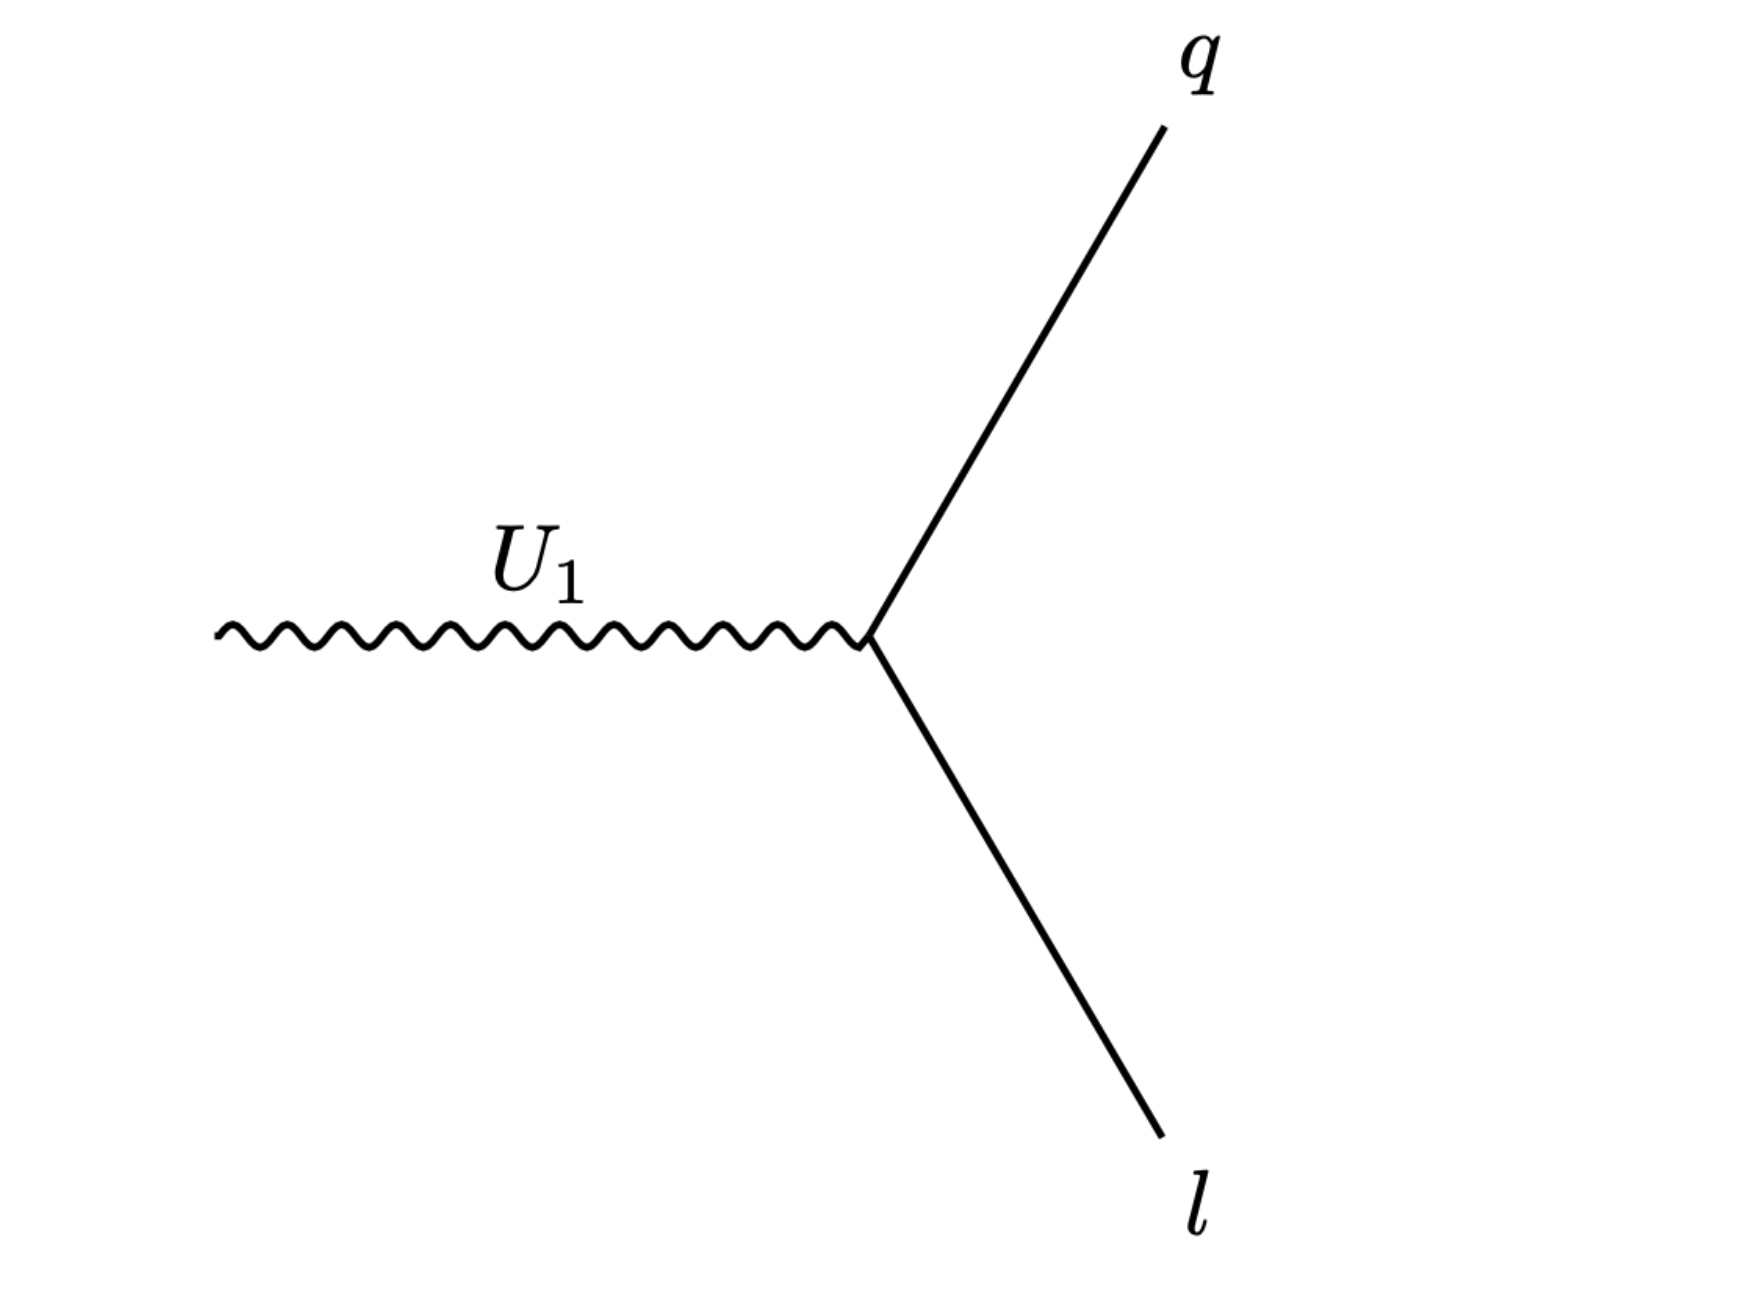
\includegraphics[width = 0.5\textwidth]{images/lq-vertex.png}
    \caption{Feynman diagram vertex showing a vector leptoquark ($U_1$) coupling to a quark $q$ and a lepton $l$.}
    \label{fig:vertex}
\end{figure}


